\documentclass[1p]{elsarticle_modified}
%\bibliographystyle{elsarticle-num}

%\usepackage[colorlinks]{hyperref}
%\usepackage{abbrmath_seonhwa} %\Abb, \Ascr, \Acal ,\Abf, \Afrak
\usepackage{amsfonts}
\usepackage{amssymb}
\usepackage{amsmath}
\usepackage{amsthm}
\usepackage{scalefnt}
\usepackage{amsbsy}
\usepackage{kotex}
\usepackage{caption}
\usepackage{subfig}
\usepackage{color}
\usepackage{graphicx}
\usepackage{xcolor} %% white, black, red, green, blue, cyan, magenta, yellow
\usepackage{float}
\usepackage{setspace}
\usepackage{hyperref}

\usepackage{tikz}
\usetikzlibrary{arrows}

\usepackage{multirow}
\usepackage{array} % fixed length table
\usepackage{hhline}

%%%%%%%%%%%%%%%%%%%%%
\makeatletter
\renewcommand*\env@matrix[1][\arraystretch]{%
	\edef\arraystretch{#1}%
	\hskip -\arraycolsep
	\let\@ifnextchar\new@ifnextchar
	\array{*\c@MaxMatrixCols c}}
\makeatother %https://tex.stackexchange.com/questions/14071/how-can-i-increase-the-line-spacing-in-a-matrix
%%%%%%%%%%%%%%%

\usepackage[normalem]{ulem}

\newcommand{\msout}[1]{\ifmmode\text{\sout{\ensuremath{#1}}}\else\sout{#1}\fi}
%SOURCE: \msout is \stkout macro in https://tex.stackexchange.com/questions/20609/strikeout-in-math-mode

\newcommand{\cancel}[1]{
	\ifmmode
	{\color{red}\msout{#1}}
	\else
	{\color{red}\sout{#1}}
	\fi
}

\newcommand{\add}[1]{
	{\color{blue}\uwave{#1}}
}

\newcommand{\replace}[2]{
	\ifmmode
	{\color{red}\msout{#1}}{\color{blue}\uwave{#2}}
	\else
	{\color{red}\sout{#1}}{\color{blue}\uwave{#2}}
	\fi
}

\newcommand{\Sol}{\mathcal{S}} %segment
\newcommand{\D}{D} %diagram
\newcommand{\A}{\mathcal{A}} %arc


%%%%%%%%%%%%%%%%%%%%%%%%%%%%%5 test

\def\sl{\operatorname{\textup{SL}}(2,\Cbb)}
\def\psl{\operatorname{\textup{PSL}}(2,\Cbb)}
\def\quan{\mkern 1mu \triangleright \mkern 1mu}

\theoremstyle{definition}
\newtheorem{thm}{Theorem}[section]
\newtheorem{prop}[thm]{Proposition}
\newtheorem{lem}[thm]{Lemma}
\newtheorem{ques}[thm]{Question}
\newtheorem{cor}[thm]{Corollary}
\newtheorem{defn}[thm]{Definition}
\newtheorem{exam}[thm]{Example}
\newtheorem{rmk}[thm]{Remark}
\newtheorem{alg}[thm]{Algorithm}

\newcommand{\I}{\sqrt{-1}}
\begin{document}

%\begin{frontmatter}
%
%\title{Boundary parabolic representations of knots up to 8 crossings}
%
%%% Group authors per affiliation:
%\author{Yunhi Cho} 
%\address{Department of Mathematics, University of Seoul, Seoul, Korea}
%\ead{yhcho@uos.ac.kr}
%
%
%\author{Seonhwa Kim} %\fnref{s_kim}}
%\address{Center for Geometry and Physics, Institute for Basic Science, Pohang, 37673, Korea}
%\ead{ryeona17@ibs.re.kr}
%
%\author{Hyuk Kim}
%\address{Department of Mathematical Sciences, Seoul National University, Seoul 08826, Korea}
%\ead{hyukkim@snu.ac.kr}
%
%\author{Seokbeom Yoon}
%\address{Department of Mathematical Sciences, Seoul National University, Seoul, 08826,  Korea}
%\ead{sbyoon15@snu.ac.kr}
%
%\begin{abstract}
%We find all boundary parabolic representation of knots up to 8 crossings.
%
%\end{abstract}
%\begin{keyword}
%    \MSC[2010] 57M25 
%\end{keyword}
%
%\end{frontmatter}

%\linenumbers
%\tableofcontents
%
\newcommand\colored[1]{\textcolor{white}{\rule[-0.35ex]{0.8em}{1.4ex}}\kern-0.8em\color{red} #1}%
%\newcommand\colored[1]{\textcolor{white}{ #1}\kern-2.17ex	\textcolor{white}{ #1}\kern-1.81ex	\textcolor{white}{ #1}\kern-2.15ex\color{red}#1	}

{\Large $\underline{12a_{1027}~(K12a_{1027})}$}

\setlength{\tabcolsep}{10pt}
\renewcommand{\arraystretch}{1.6}
\vspace{1cm}\begin{tabular}{m{100pt}>{\centering\arraybackslash}m{274pt}}
\multirow{5}{120pt}{
	\centering
	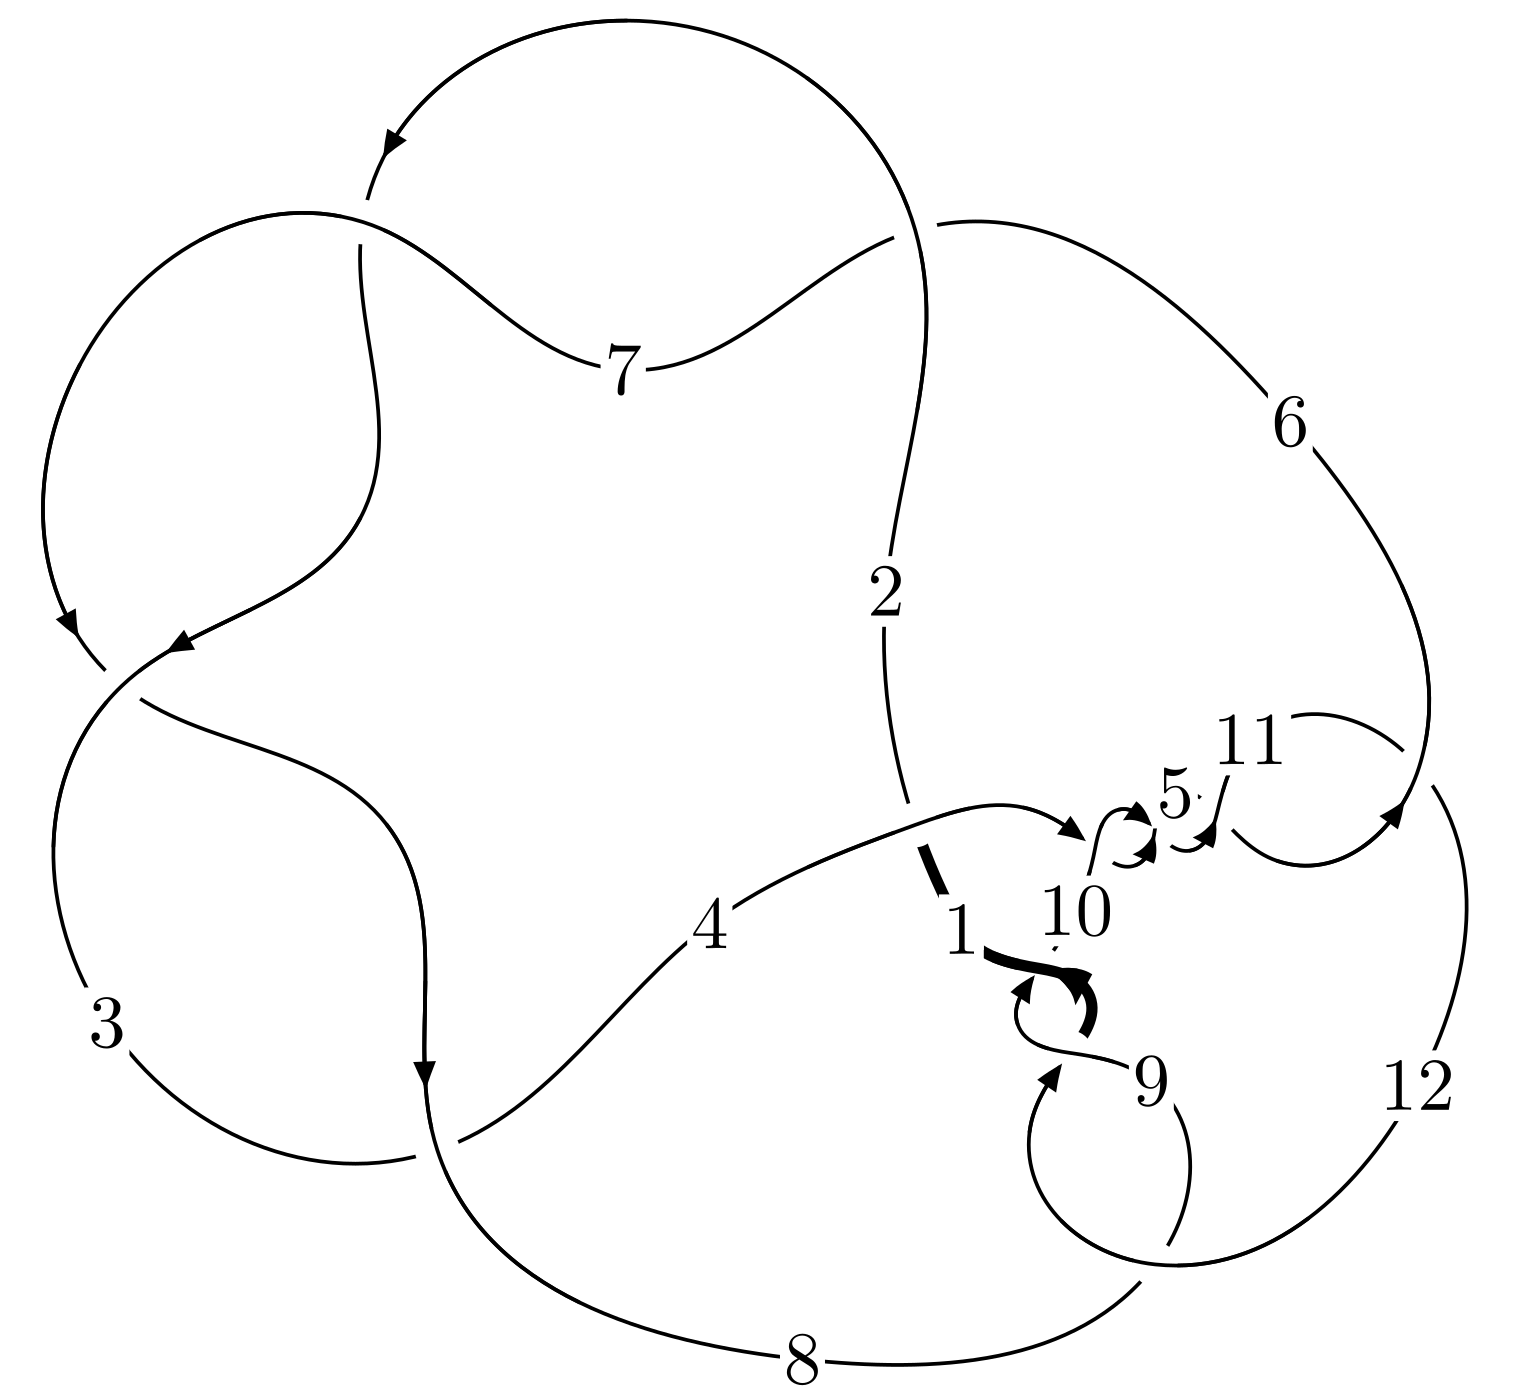
\includegraphics[width=112pt]{../../../GIT/diagram.site/Diagrams/png/1828_12a_1027.png}\\
\ \ \ A knot diagram\footnotemark}&
\allowdisplaybreaks
\textbf{Linearized knot diagam} \\
\cline{2-2}
 &
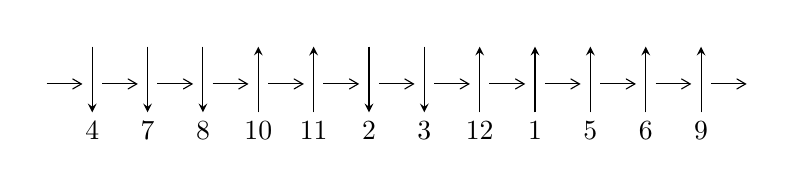
\begin{tikzpicture}[x=20pt, y=17pt]
	% nodes
	\node (C0) at (0, 0) {};
	\node (C1) at (1, 0) {};
	\node (C1U) at (1, +1) {};
	\node (C1D) at (1, -1) {4};

	\node (C2) at (2, 0) {};
	\node (C2U) at (2, +1) {};
	\node (C2D) at (2, -1) {7};

	\node (C3) at (3, 0) {};
	\node (C3U) at (3, +1) {};
	\node (C3D) at (3, -1) {8};

	\node (C4) at (4, 0) {};
	\node (C4U) at (4, +1) {};
	\node (C4D) at (4, -1) {10};

	\node (C5) at (5, 0) {};
	\node (C5U) at (5, +1) {};
	\node (C5D) at (5, -1) {11};

	\node (C6) at (6, 0) {};
	\node (C6U) at (6, +1) {};
	\node (C6D) at (6, -1) {2};

	\node (C7) at (7, 0) {};
	\node (C7U) at (7, +1) {};
	\node (C7D) at (7, -1) {3};

	\node (C8) at (8, 0) {};
	\node (C8U) at (8, +1) {};
	\node (C8D) at (8, -1) {12};

	\node (C9) at (9, 0) {};
	\node (C9U) at (9, +1) {};
	\node (C9D) at (9, -1) {1};

	\node (C10) at (10, 0) {};
	\node (C10U) at (10, +1) {};
	\node (C10D) at (10, -1) {5};

	\node (C11) at (11, 0) {};
	\node (C11U) at (11, +1) {};
	\node (C11D) at (11, -1) {6};

	\node (C12) at (12, 0) {};
	\node (C12U) at (12, +1) {};
	\node (C12D) at (12, -1) {9};
	\node (C13) at (13, 0) {};

	% arrows
	\draw[->,>={angle 60}]
	(C0) edge (C1) (C1) edge (C2) (C2) edge (C3) (C3) edge (C4) (C4) edge (C5) (C5) edge (C6) (C6) edge (C7) (C7) edge (C8) (C8) edge (C9) (C9) edge (C10) (C10) edge (C11) (C11) edge (C12) (C12) edge (C13) ;	\draw[->,>=stealth]
	(C1U) edge (C1D) (C2U) edge (C2D) (C3U) edge (C3D) (C4D) edge (C4U) (C5D) edge (C5U) (C6U) edge (C6D) (C7U) edge (C7D) (C8D) edge (C8U) (C9D) edge (C9U) (C10D) edge (C10U) (C11D) edge (C11U) (C12D) edge (C12U) ;
	\end{tikzpicture} \\
\hhline{~~} \\& 
\textbf{Solving Sequence} \\ \cline{2-2} 
 &
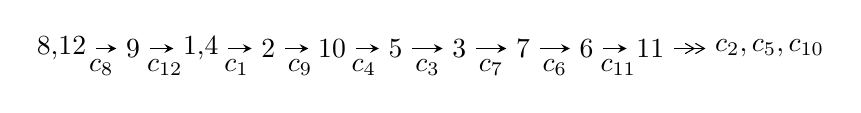
\begin{tikzpicture}[x=23pt, y=7pt]
	% node
	\node (A0) at (-1/8, 0) {8,12};
	\node (A1) at (1, 0) {9};
	\node (A2) at (33/16, 0) {1,4};
	\node (A3) at (25/8, 0) {2};
	\node (A4) at (33/8, 0) {10};
	\node (A5) at (41/8, 0) {5};
	\node (A6) at (49/8, 0) {3};
	\node (A7) at (57/8, 0) {7};
	\node (A8) at (65/8, 0) {6};
	\node (A9) at (73/8, 0) {11};
	\node (C1) at (1/2, -1) {$c_{8}$};
	\node (C2) at (3/2, -1) {$c_{12}$};
	\node (C3) at (21/8, -1) {$c_{1}$};
	\node (C4) at (29/8, -1) {$c_{9}$};
	\node (C5) at (37/8, -1) {$c_{4}$};
	\node (C6) at (45/8, -1) {$c_{3}$};
	\node (C7) at (53/8, -1) {$c_{7}$};
	\node (C8) at (61/8, -1) {$c_{6}$};
	\node (C9) at (69/8, -1) {$c_{11}$};
	\node (A10) at (11, 0) {$c_{2},c_{5},c_{10}$};

	% edge
	\draw[->,>=stealth]	
	(A0) edge (A1) (A1) edge (A2) (A2) edge (A3) (A3) edge (A4) (A4) edge (A5) (A5) edge (A6) (A6) edge (A7) (A7) edge (A8) (A8) edge (A9) ;
	\draw[->>,>={angle 60}]	
	(A9) edge (A10);
\end{tikzpicture} \\ 

\end{tabular} \\

\footnotetext{
The image of knot diagram is generated by the software ``\textbf{Draw programme}" developed by Andrew Bartholomew(\url{http://www.layer8.co.uk/maths/draw/index.htm\#Running-draw}), where we modified some parts for our purpose(\url{https://github.com/CATsTAILs/LinksPainter}).
}\phantom \\ \newline 
\centering \textbf{Ideals for irreducible components\footnotemark of $X_{\text{par}}$} 
 
\begin{align*}
I^u_{1}&=\langle 
-5.36041\times10^{31} u^{46}-1.13554\times10^{32} u^{45}+\cdots+1.29302\times10^{32} b-1.94404\times10^{32},\\
\phantom{I^u_{1}}&\phantom{= \langle  }2.24156\times10^{31} u^{46}+7.53273\times10^{31} u^{45}+\cdots+3.23255\times10^{31} a+5.49837\times10^{32},\;u^{47}+3 u^{46}+\cdots+11 u+1\rangle \\
I^u_{2}&=\langle 
b^2- b-1,\;a,\;u+1\rangle \\
I^u_{3}&=\langle 
b^2+b-1,\;a^2-2,\;u-1\rangle \\
\\
\end{align*}
\raggedright * 3 irreducible components of $\dim_{\mathbb{C}}=0$, with total 53 representations.\\
\footnotetext{All coefficients of polynomials are rational numbers. But the coefficients are sometimes approximated in decimal forms when there is not enough margin.}
\newpage
\renewcommand{\arraystretch}{1}
\centering \section*{I. $I^u_{1}= \langle -5.36\times10^{31} u^{46}-1.14\times10^{32} u^{45}+\cdots+1.29\times10^{32} b-1.94\times10^{32},\;2.24\times10^{31} u^{46}+7.53\times10^{31} u^{45}+\cdots+3.23\times10^{31} a+5.50\times10^{32},\;u^{47}+3 u^{46}+\cdots+11 u+1 \rangle$}
\flushleft \textbf{(i) Arc colorings}\\
\begin{tabular}{m{7pt} m{180pt} m{7pt} m{180pt} }
\flushright $a_{8}=$&$\begin{pmatrix}1\\0\end{pmatrix}$ \\
\flushright $a_{12}=$&$\begin{pmatrix}0\\u\end{pmatrix}$ \\
\flushright $a_{9}=$&$\begin{pmatrix}1\\- u^2\end{pmatrix}$ \\
\flushright $a_{1}=$&$\begin{pmatrix}u\\- u^3+u\end{pmatrix}$ \\
\flushright $a_{4}=$&$\begin{pmatrix}-0.693436 u^{46}-2.33028 u^{45}+\cdots+51.8733 u-17.0094\\0.414565 u^{46}+0.878210 u^{45}+\cdots-2.42558 u+1.50349\end{pmatrix}$ \\
\flushright $a_{2}=$&$\begin{pmatrix}1.27062 u^{46}+4.66656 u^{45}+\cdots-92.6821 u+25.3900\\-1.34352 u^{46}-2.38910 u^{45}+\cdots-1.23584 u-2.87972\end{pmatrix}$ \\
\flushright $a_{10}=$&$\begin{pmatrix}- u^2+1\\u^4-2 u^2\end{pmatrix}$ \\
\flushright $a_{5}=$&$\begin{pmatrix}-0.269337 u^{46}-1.48602 u^{45}+\cdots+49.2076 u-15.7275\\0.532338 u^{46}+1.05855 u^{45}+\cdots-1.02870 u+1.61606\end{pmatrix}$ \\
\flushright $a_{3}=$&$\begin{pmatrix}-0.278871 u^{46}-1.45207 u^{45}+\cdots+49.4477 u-15.5059\\0.414565 u^{46}+0.878210 u^{45}+\cdots-2.42558 u+1.50349\end{pmatrix}$ \\
\flushright $a_{7}=$&$\begin{pmatrix}1.09240 u^{46}+4.31714 u^{45}+\cdots-94.1022 u+24.9244\\-1.00057 u^{46}-1.67329 u^{45}+\cdots-1.56609 u-2.90262\end{pmatrix}$ \\
\flushright $a_{6}=$&$\begin{pmatrix}-0.741274 u^{46}-2.48932 u^{45}+\cdots+48.4395 u-16.5010\\1.01218 u^{46}+1.69492 u^{45}+\cdots+0.702410 u+1.76957\end{pmatrix}$ \\
\flushright $a_{11}=$&$\begin{pmatrix}2.45199 u^{46}+6.38937 u^{45}+\cdots-77.9752 u+22.6332\\0.951398 u^{46}+1.42569 u^{45}+\cdots+12.6443 u-1.14744\end{pmatrix}$\\&\end{tabular}
\flushleft \textbf{(ii) Obstruction class $= -1$}\\~\\
\flushleft \textbf{(iii) Cusp Shapes $= 0.0277644 u^{46}-0.160999 u^{45}+\cdots-5.16637 u-2.38003$}\\~\\
\newpage\renewcommand{\arraystretch}{1}
\flushleft \textbf{(iv) u-Polynomials at the component}\newline \\
\begin{tabular}{m{50pt}|m{274pt}}
Crossings & \hspace{64pt}u-Polynomials at each crossing \\
\hline $$\begin{aligned}c_{1}\end{aligned}$$&$\begin{aligned}
&u^{47}-10 u^{46}+\cdots-1252 u-41
\end{aligned}$\\
\hline $$\begin{aligned}c_{2},c_{3},c_{6}\\c_{7}\end{aligned}$$&$\begin{aligned}
&u^{47}-2 u^{46}+\cdots-10 u+1
\end{aligned}$\\
\hline $$\begin{aligned}c_{4},c_{5},c_{10}\\c_{11}\end{aligned}$$&$\begin{aligned}
&u^{47}- u^{46}+\cdots-4 u+4
\end{aligned}$\\
\hline $$\begin{aligned}c_{8},c_{9},c_{12}\end{aligned}$$&$\begin{aligned}
&u^{47}-3 u^{46}+\cdots+11 u-1
\end{aligned}$\\
\hline
\end{tabular}\\~\\
\newpage\renewcommand{\arraystretch}{1}
\flushleft \textbf{(v) Riley Polynomials at the component}\newline \\
\begin{tabular}{m{50pt}|m{274pt}}
Crossings & \hspace{64pt}Riley Polynomials at each crossing \\
\hline $$\begin{aligned}c_{1}\end{aligned}$$&$\begin{aligned}
&y^{47}+18 y^{46}+\cdots+1361766 y-1681
\end{aligned}$\\
\hline $$\begin{aligned}c_{2},c_{3},c_{6}\\c_{7}\end{aligned}$$&$\begin{aligned}
&y^{47}-54 y^{46}+\cdots+74 y-1
\end{aligned}$\\
\hline $$\begin{aligned}c_{4},c_{5},c_{10}\\c_{11}\end{aligned}$$&$\begin{aligned}
&y^{47}-57 y^{46}+\cdots+304 y-16
\end{aligned}$\\
\hline $$\begin{aligned}c_{8},c_{9},c_{12}\end{aligned}$$&$\begin{aligned}
&y^{47}-47 y^{46}+\cdots+211 y-1
\end{aligned}$\\
\hline
\end{tabular}\\~\\
\newpage\flushleft \textbf{(vi) Complex Volumes and Cusp Shapes}
$$\begin{array}{c|c|c}  
\text{Solutions to }I^u_{1}& \I (\text{vol} + \sqrt{-1}CS) & \text{Cusp shape}\\
 \hline 
\begin{aligned}
u &= \phantom{-}0.384168 + 0.933735 I \\
a &= -1.12092 - 1.02399 I \\
b &= -1.55340 + 0.17162 I\end{aligned}
 & \phantom{-}1.07008 + 7.34464 I & \phantom{-}2.44287 - 4.66692 I \\ \hline\begin{aligned}
u &= \phantom{-}0.384168 - 0.933735 I \\
a &= -1.12092 + 1.02399 I \\
b &= -1.55340 - 0.17162 I\end{aligned}
 & \phantom{-}1.07008 - 7.34464 I & \phantom{-}2.44287 + 4.66692 I \\ \hline\begin{aligned}
u &= \phantom{-}0.655220 + 0.738260 I \\
a &= -0.024512 - 0.284636 I \\
b &= \phantom{-}0.394578 + 0.582858 I\end{aligned}
 & \phantom{-}8.68282 + 0.69167 I & \phantom{-}7.69697 + 0.39730 I \\ \hline\begin{aligned}
u &= \phantom{-}0.655220 - 0.738260 I \\
a &= -0.024512 + 0.284636 I \\
b &= \phantom{-}0.394578 - 0.582858 I\end{aligned}
 & \phantom{-}8.68282 - 0.69167 I & \phantom{-}7.69697 - 0.39730 I \\ \hline\begin{aligned}
u &= \phantom{-}0.500977 + 0.840491 I \\
a &= \phantom{-}0.619681 + 0.697367 I \\
b &= \phantom{-}0.573333 - 0.570047 I\end{aligned}
 & \phantom{-}8.15872 + 4.64474 I & \phantom{-}5.91649 - 5.94308 I \\ \hline\begin{aligned}
u &= \phantom{-}0.500977 - 0.840491 I \\
a &= \phantom{-}0.619681 - 0.697367 I \\
b &= \phantom{-}0.573333 + 0.570047 I\end{aligned}
 & \phantom{-}8.15872 - 4.64474 I & \phantom{-}5.91649 + 5.94308 I \\ \hline\begin{aligned}
u &= \phantom{-}1.05786\phantom{ +0.000000I} \\
a &= \phantom{-}1.39495\phantom{ +0.000000I} \\
b &= -0.132955\phantom{ +0.000000I}\end{aligned}
 & \phantom{-}6.53482\phantom{ +0.000000I} & \phantom{-}14.2750\phantom{ +0.000000I} \\ \hline\begin{aligned}
u &= -0.808561 + 0.480294 I \\
a &= \phantom{-}0.244914 - 0.563300 I \\
b &= \phantom{-}1.53534 - 0.04664 I\end{aligned}
 & -5.40245 + 0.60387 I & \phantom{-}2.86876 - 0.80089 I \\ \hline\begin{aligned}
u &= -0.808561 - 0.480294 I \\
a &= \phantom{-}0.244914 + 0.563300 I \\
b &= \phantom{-}1.53534 + 0.04664 I\end{aligned}
 & -5.40245 - 0.60387 I & \phantom{-}2.86876 + 0.80089 I \\ \hline\begin{aligned}
u &= \phantom{-}0.897365 + 0.697135 I \\
a &= -0.520554 - 0.385254 I \\
b &= -1.47865 - 0.13246 I\end{aligned}
 & \phantom{-}2.62151 - 1.72568 I & \phantom{-}4.31042 + 0.20195 I\\
 \hline 
 \end{array}$$\newpage$$\begin{array}{c|c|c}  
\text{Solutions to }I^u_{1}& \I (\text{vol} + \sqrt{-1}CS) & \text{Cusp shape}\\
 \hline 
\begin{aligned}
u &= \phantom{-}0.897365 - 0.697135 I \\
a &= -0.520554 + 0.385254 I \\
b &= -1.47865 + 0.13246 I\end{aligned}
 & \phantom{-}2.62151 + 1.72568 I & \phantom{-}4.31042 - 0.20195 I \\ \hline\begin{aligned}
u &= -0.860635\phantom{ +0.000000I} \\
a &= -0.263406\phantom{ +0.000000I} \\
b &= -0.380700\phantom{ +0.000000I}\end{aligned}
 & \phantom{-}1.06395\phantom{ +0.000000I} & \phantom{-}15.0300\phantom{ +0.000000I} \\ \hline\begin{aligned}
u &= -0.347438 + 0.773858 I \\
a &= \phantom{-}1.05026 - 1.26332 I \\
b &= \phantom{-}1.55717 + 0.11542 I\end{aligned}
 & -6.84691 - 5.11929 I & -0.37879 + 6.36237 I \\ \hline\begin{aligned}
u &= -0.347438 - 0.773858 I \\
a &= \phantom{-}1.05026 + 1.26332 I \\
b &= \phantom{-}1.55717 - 0.11542 I\end{aligned}
 & -6.84691 + 5.11929 I & -0.37879 - 6.36237 I \\ \hline\begin{aligned}
u &= \phantom{-}1.17129\phantom{ +0.000000I} \\
a &= -0.134391\phantom{ +0.000000I} \\
b &= -1.65236\phantom{ +0.000000I}\end{aligned}
 & -6.66969\phantom{ +0.000000I} & \phantom{-}8.57260\phantom{ +0.000000I} \\ \hline\begin{aligned}
u &= -0.375308 + 0.614572 I \\
a &= -0.633040 + 0.852370 I \\
b &= -0.568261 - 0.421058 I\end{aligned}
 & \phantom{-}0.32221 - 3.19990 I & \phantom{-}3.06029 + 9.19456 I \\ \hline\begin{aligned}
u &= -0.375308 - 0.614572 I \\
a &= -0.633040 - 0.852370 I \\
b &= -0.568261 + 0.421058 I\end{aligned}
 & \phantom{-}0.32221 + 3.19990 I & \phantom{-}3.06029 - 9.19456 I \\ \hline\begin{aligned}
u &= \phantom{-}1.28718\phantom{ +0.000000I} \\
a &= -0.273773\phantom{ +0.000000I} \\
b &= \phantom{-}0.949055\phantom{ +0.000000I}\end{aligned}
 & \phantom{-}2.25442\phantom{ +0.000000I} & \phantom{-}5.01370\phantom{ +0.000000I} \\ \hline\begin{aligned}
u &= \phantom{-}0.337492 + 0.539565 I \\
a &= -0.60781 - 1.74002 I \\
b &= -1.56840 + 0.05663 I\end{aligned}
 & -8.40867 + 1.57482 I & -4.99229 - 1.00293 I \\ \hline\begin{aligned}
u &= \phantom{-}0.337492 - 0.539565 I \\
a &= -0.60781 + 1.74002 I \\
b &= -1.56840 - 0.05663 I\end{aligned}
 & -8.40867 - 1.57482 I & -4.99229 + 1.00293 I\\
 \hline 
 \end{array}$$\newpage$$\begin{array}{c|c|c}  
\text{Solutions to }I^u_{1}& \I (\text{vol} + \sqrt{-1}CS) & \text{Cusp shape}\\
 \hline 
\begin{aligned}
u &= -1.39429\phantom{ +0.000000I} \\
a &= \phantom{-}0.234243\phantom{ +0.000000I} \\
b &= \phantom{-}1.70918\phantom{ +0.000000I}\end{aligned}
 & \phantom{-}0.706458\phantom{ +0.000000I} & \phantom{-0.000000 } 0 \\ \hline\begin{aligned}
u &= -0.480504 + 0.364841 I \\
a &= \phantom{-}0.028159 - 0.293507 I \\
b &= -0.310058 + 0.354613 I\end{aligned}
 & \phantom{-}1.036960 - 0.314856 I & \phantom{-}8.23983 + 0.59404 I \\ \hline\begin{aligned}
u &= -0.480504 - 0.364841 I \\
a &= \phantom{-}0.028159 + 0.293507 I \\
b &= -0.310058 - 0.354613 I\end{aligned}
 & \phantom{-}1.036960 + 0.314856 I & \phantom{-}8.23983 - 0.59404 I \\ \hline\begin{aligned}
u &= -1.398200 + 0.068490 I \\
a &= -0.31034 - 1.47254 I \\
b &= \phantom{-}0.490370 + 0.539803 I\end{aligned}
 & \phantom{-}3.97392 - 1.86699 I & \phantom{-0.000000 } 0 \\ \hline\begin{aligned}
u &= -1.398200 - 0.068490 I \\
a &= -0.31034 + 1.47254 I \\
b &= \phantom{-}0.490370 - 0.539803 I\end{aligned}
 & \phantom{-}3.97392 + 1.86699 I & \phantom{-0.000000 } 0 \\ \hline\begin{aligned}
u &= \phantom{-}1.42950 + 0.07034 I \\
a &= -1.27663 + 0.73949 I \\
b &= \phantom{-}1.44285 - 0.09561 I\end{aligned}
 & \phantom{-}1.56798 + 0.38836 I & \phantom{-0.000000 } 0 \\ \hline\begin{aligned}
u &= \phantom{-}1.42950 - 0.07034 I \\
a &= -1.27663 - 0.73949 I \\
b &= \phantom{-}1.44285 + 0.09561 I\end{aligned}
 & \phantom{-}1.56798 - 0.38836 I & \phantom{-0.000000 } 0 \\ \hline\begin{aligned}
u &= -1.42981 + 0.19455 I \\
a &= \phantom{-}0.91947 + 1.50523 I \\
b &= -1.52603 - 0.14762 I\end{aligned}
 & -2.72276 - 4.28492 I & \phantom{-0.000000 } 0 \\ \hline\begin{aligned}
u &= -1.42981 - 0.19455 I \\
a &= \phantom{-}0.91947 - 1.50523 I \\
b &= -1.52603 + 0.14762 I\end{aligned}
 & -2.72276 + 4.28492 I & \phantom{-0.000000 } 0 \\ \hline\begin{aligned}
u &= \phantom{-}1.44250 + 0.10539 I \\
a &= \phantom{-}0.421487 + 1.174390 I \\
b &= -0.340123 - 0.621543 I\end{aligned}
 & \phantom{-}7.07024 + 2.02020 I & \phantom{-0.000000 } 0\\
 \hline 
 \end{array}$$\newpage$$\begin{array}{c|c|c}  
\text{Solutions to }I^u_{1}& \I (\text{vol} + \sqrt{-1}CS) & \text{Cusp shape}\\
 \hline 
\begin{aligned}
u &= \phantom{-}1.44250 - 0.10539 I \\
a &= \phantom{-}0.421487 - 1.174390 I \\
b &= -0.340123 + 0.621543 I\end{aligned}
 & \phantom{-}7.07024 - 2.02020 I & \phantom{-0.000000 } 0 \\ \hline\begin{aligned}
u &= \phantom{-}1.45842 + 0.19966 I \\
a &= \phantom{-}0.02427 - 1.46022 I \\
b &= -0.613332 + 0.585418 I\end{aligned}
 & \phantom{-}6.27479 + 6.12368 I & \phantom{-0.000000 } 0 \\ \hline\begin{aligned}
u &= \phantom{-}1.45842 - 0.19966 I \\
a &= \phantom{-}0.02427 + 1.46022 I \\
b &= -0.613332 - 0.585418 I\end{aligned}
 & \phantom{-}6.27479 - 6.12368 I & \phantom{-0.000000 } 0 \\ \hline\begin{aligned}
u &= \phantom{-}1.46180 + 0.28357 I \\
a &= -0.45847 + 1.62265 I \\
b &= \phantom{-}1.56761 - 0.18045 I\end{aligned}
 & -1.00497 + 8.94411 I & \phantom{-0.000000 } 0 \\ \hline\begin{aligned}
u &= \phantom{-}1.46180 - 0.28357 I \\
a &= -0.45847 - 1.62265 I \\
b &= \phantom{-}1.56761 + 0.18045 I\end{aligned}
 & -1.00497 - 8.94411 I & \phantom{-0.000000 } 0 \\ \hline\begin{aligned}
u &= -1.50841 + 0.35834 I \\
a &= \phantom{-}0.14634 + 1.54270 I \\
b &= -1.60053 - 0.20896 I\end{aligned}
 & \phantom{-}7.16899 - 12.03310 I & \phantom{-0.000000 } 0 \\ \hline\begin{aligned}
u &= -1.50841 - 0.35834 I \\
a &= \phantom{-}0.14634 - 1.54270 I \\
b &= -1.60053 + 0.20896 I\end{aligned}
 & \phantom{-}7.16899 + 12.03310 I & \phantom{-0.000000 } 0 \\ \hline\begin{aligned}
u &= -1.55108 + 0.09583 I \\
a &= \phantom{-}0.399380 - 0.446871 I \\
b &= -1.235980 + 0.286169 I\end{aligned}
 & \phantom{-}11.18770 - 0.40908 I & \phantom{-0.000000 } 0 \\ \hline\begin{aligned}
u &= -1.55108 - 0.09583 I \\
a &= \phantom{-}0.399380 + 0.446871 I \\
b &= -1.235980 - 0.286169 I\end{aligned}
 & \phantom{-}11.18770 + 0.40908 I & \phantom{-0.000000 } 0 \\ \hline\begin{aligned}
u &= -1.54096 + 0.29431 I \\
a &= \phantom{-}0.118024 - 1.335240 I \\
b &= \phantom{-}0.690898 + 0.651096 I\end{aligned}
 & \phantom{-}14.8277 - 8.8002 I & \phantom{-0.000000 } 0\\
 \hline 
 \end{array}$$\newpage$$\begin{array}{c|c|c}  
\text{Solutions to }I^u_{1}& \I (\text{vol} + \sqrt{-1}CS) & \text{Cusp shape}\\
 \hline 
\begin{aligned}
u &= -1.54096 - 0.29431 I \\
a &= \phantom{-}0.118024 + 1.335240 I \\
b &= \phantom{-}0.690898 - 0.651096 I\end{aligned}
 & \phantom{-}14.8277 + 8.8002 I & \phantom{-0.000000 } 0 \\ \hline\begin{aligned}
u &= -1.56276 + 0.21755 I \\
a &= -0.336855 + 1.023130 I \\
b &= \phantom{-}0.291108 - 0.752857 I\end{aligned}
 & \phantom{-}16.0174 - 4.1262 I & \phantom{-0.000000 } 0 \\ \hline\begin{aligned}
u &= -1.56276 - 0.21755 I \\
a &= -0.336855 - 1.023130 I \\
b &= \phantom{-}0.291108 + 0.752857 I\end{aligned}
 & \phantom{-}16.0174 + 4.1262 I & \phantom{-0.000000 } 0 \\ \hline\begin{aligned}
u &= \phantom{-}0.168164 + 0.305680 I \\
a &= \phantom{-}0.47692 + 1.60928 I \\
b &= \phantom{-}0.579305 - 0.209601 I\end{aligned}
 & -1.053100 + 0.603352 I & -5.28744 - 1.90691 I \\ \hline\begin{aligned}
u &= \phantom{-}0.168164 - 0.305680 I \\
a &= \phantom{-}0.47692 - 1.60928 I \\
b &= \phantom{-}0.579305 + 0.209601 I\end{aligned}
 & -1.053100 - 0.603352 I & -5.28744 + 1.90691 I \\ \hline\begin{aligned}
u &= \phantom{-}0.343456\phantom{ +0.000000I} \\
a &= -3.57272\phantom{ +0.000000I} \\
b &= -0.759828\phantom{ +0.000000I}\end{aligned}
 & \phantom{-}4.20368\phantom{ +0.000000I} & -1.73630\phantom{ +0.000000I} \\ \hline\begin{aligned}
u &= -0.0700122\phantom{ +0.000000I} \\
a &= -20.7044\phantom{ +0.000000I} \\
b &= \phantom{-}1.61200\phantom{ +0.000000I}\end{aligned}
 & -3.93845\phantom{ +0.000000I} & -2.00240\phantom{ +0.000000I}\\
 \hline 
 \end{array}$$\newpage\newpage\renewcommand{\arraystretch}{1}
\centering \section*{II. $I^u_{2}= \langle b^2- b-1,\;a,\;u+1 \rangle$}
\flushleft \textbf{(i) Arc colorings}\\
\begin{tabular}{m{7pt} m{180pt} m{7pt} m{180pt} }
\flushright $a_{8}=$&$\begin{pmatrix}1\\0\end{pmatrix}$ \\
\flushright $a_{12}=$&$\begin{pmatrix}0\\-1\end{pmatrix}$ \\
\flushright $a_{9}=$&$\begin{pmatrix}1\\-1\end{pmatrix}$ \\
\flushright $a_{1}=$&$\begin{pmatrix}-1\\0\end{pmatrix}$ \\
\flushright $a_{4}=$&$\begin{pmatrix}0\\b\end{pmatrix}$ \\
\flushright $a_{2}=$&$\begin{pmatrix}-1\\- b-1\end{pmatrix}$ \\
\flushright $a_{10}=$&$\begin{pmatrix}0\\-1\end{pmatrix}$ \\
\flushright $a_{5}=$&$\begin{pmatrix}0\\b\end{pmatrix}$ \\
\flushright $a_{3}=$&$\begin{pmatrix}b\\b\end{pmatrix}$ \\
\flushright $a_{7}=$&$\begin{pmatrix}- b\\- b-1\end{pmatrix}$ \\
\flushright $a_{6}=$&$\begin{pmatrix}0\\b\end{pmatrix}$ \\
\flushright $a_{11}=$&$\begin{pmatrix}0\\-1\end{pmatrix}$\\&\end{tabular}
\flushleft \textbf{(ii) Obstruction class $= 1$}\\~\\
\flushleft \textbf{(iii) Cusp Shapes $= -6$}\\~\\
\newpage\renewcommand{\arraystretch}{1}
\flushleft \textbf{(iv) u-Polynomials at the component}\newline \\
\begin{tabular}{m{50pt}|m{274pt}}
Crossings & \hspace{64pt}u-Polynomials at each crossing \\
\hline $$\begin{aligned}c_{1},c_{2},c_{3}\end{aligned}$$&$\begin{aligned}
&u^2+u-1
\end{aligned}$\\
\hline $$\begin{aligned}c_{4},c_{5},c_{10}\\c_{11}\end{aligned}$$&$\begin{aligned}
&u^2
\end{aligned}$\\
\hline $$\begin{aligned}c_{6},c_{7}\end{aligned}$$&$\begin{aligned}
&u^2- u-1
\end{aligned}$\\
\hline $$\begin{aligned}c_{8},c_{9}\end{aligned}$$&$\begin{aligned}
&(u+1)^2
\end{aligned}$\\
\hline $$\begin{aligned}c_{12}\end{aligned}$$&$\begin{aligned}
&(u-1)^2
\end{aligned}$\\
\hline
\end{tabular}\\~\\
\newpage\renewcommand{\arraystretch}{1}
\flushleft \textbf{(v) Riley Polynomials at the component}\newline \\
\begin{tabular}{m{50pt}|m{274pt}}
Crossings & \hspace{64pt}Riley Polynomials at each crossing \\
\hline $$\begin{aligned}c_{1},c_{2},c_{3}\\c_{6},c_{7}\end{aligned}$$&$\begin{aligned}
&y^2-3 y+1
\end{aligned}$\\
\hline $$\begin{aligned}c_{4},c_{5},c_{10}\\c_{11}\end{aligned}$$&$\begin{aligned}
&y^2
\end{aligned}$\\
\hline $$\begin{aligned}c_{8},c_{9},c_{12}\end{aligned}$$&$\begin{aligned}
&(y-1)^2
\end{aligned}$\\
\hline
\end{tabular}\\~\\
\newpage\flushleft \textbf{(vi) Complex Volumes and Cusp Shapes}
$$\begin{array}{c|c|c}  
\text{Solutions to }I^u_{2}& \I (\text{vol} + \sqrt{-1}CS) & \text{Cusp shape}\\
 \hline 
\begin{aligned}
u &= -1.00000\phantom{ +0.000000I} \\
a &= \phantom{-0.000000 } 0 \\
b &= -0.618034\phantom{ +0.000000I}\end{aligned}
 & \phantom{-}0.657974\phantom{ +0.000000I} & -6.00000\phantom{ +0.000000I} \\ \hline\begin{aligned}
u &= -1.00000\phantom{ +0.000000I} \\
a &= \phantom{-0.000000 } 0 \\
b &= \phantom{-}1.61803\phantom{ +0.000000I}\end{aligned}
 & -7.23771\phantom{ +0.000000I} & -6.00000\phantom{ +0.000000I}\\
 \hline 
 \end{array}$$\newpage\newpage\renewcommand{\arraystretch}{1}
\centering \section*{III. $I^u_{3}= \langle b^2+b-1,\;a^2-2,\;u-1 \rangle$}
\flushleft \textbf{(i) Arc colorings}\\
\begin{tabular}{m{7pt} m{180pt} m{7pt} m{180pt} }
\flushright $a_{8}=$&$\begin{pmatrix}1\\0\end{pmatrix}$ \\
\flushright $a_{12}=$&$\begin{pmatrix}0\\1\end{pmatrix}$ \\
\flushright $a_{9}=$&$\begin{pmatrix}1\\-1\end{pmatrix}$ \\
\flushright $a_{1}=$&$\begin{pmatrix}1\\0\end{pmatrix}$ \\
\flushright $a_{4}=$&$\begin{pmatrix}a\\b\end{pmatrix}$ \\
\flushright $a_{2}=$&$\begin{pmatrix}b a+1\\- b+1\end{pmatrix}$ \\
\flushright $a_{10}=$&$\begin{pmatrix}0\\-1\end{pmatrix}$ \\
\flushright $a_{5}=$&$\begin{pmatrix}a\\b- a\end{pmatrix}$ \\
\flushright $a_{3}=$&$\begin{pmatrix}b+a\\b\end{pmatrix}$ \\
\flushright $a_{7}=$&$\begin{pmatrix}- b a+b\\b-1\end{pmatrix}$ \\
\flushright $a_{6}=$&$\begin{pmatrix}- a\\- b\end{pmatrix}$ \\
\flushright $a_{11}=$&$\begin{pmatrix}-2\\- b a+1\end{pmatrix}$\\&\end{tabular}
\flushleft \textbf{(ii) Obstruction class $= 1$}\\~\\
\flushleft \textbf{(iii) Cusp Shapes $= 4$}\\~\\
\newpage\renewcommand{\arraystretch}{1}
\flushleft \textbf{(iv) u-Polynomials at the component}\newline \\
\begin{tabular}{m{50pt}|m{274pt}}
Crossings & \hspace{64pt}u-Polynomials at each crossing \\
\hline $$\begin{aligned}c_{1},c_{6},c_{7}\end{aligned}$$&$\begin{aligned}
&(u^2+u-1)^2
\end{aligned}$\\
\hline $$\begin{aligned}c_{2},c_{3}\end{aligned}$$&$\begin{aligned}
&(u^2- u-1)^2
\end{aligned}$\\
\hline $$\begin{aligned}c_{4},c_{5},c_{10}\\c_{11}\end{aligned}$$&$\begin{aligned}
&(u^2-2)^2
\end{aligned}$\\
\hline $$\begin{aligned}c_{8},c_{9}\end{aligned}$$&$\begin{aligned}
&(u-1)^4
\end{aligned}$\\
\hline $$\begin{aligned}c_{12}\end{aligned}$$&$\begin{aligned}
&(u+1)^4
\end{aligned}$\\
\hline
\end{tabular}\\~\\
\newpage\renewcommand{\arraystretch}{1}
\flushleft \textbf{(v) Riley Polynomials at the component}\newline \\
\begin{tabular}{m{50pt}|m{274pt}}
Crossings & \hspace{64pt}Riley Polynomials at each crossing \\
\hline $$\begin{aligned}c_{1},c_{2},c_{3}\\c_{6},c_{7}\end{aligned}$$&$\begin{aligned}
&(y^2-3 y+1)^2
\end{aligned}$\\
\hline $$\begin{aligned}c_{4},c_{5},c_{10}\\c_{11}\end{aligned}$$&$\begin{aligned}
&(y-2)^4
\end{aligned}$\\
\hline $$\begin{aligned}c_{8},c_{9},c_{12}\end{aligned}$$&$\begin{aligned}
&(y-1)^4
\end{aligned}$\\
\hline
\end{tabular}\\~\\
\newpage\flushleft \textbf{(vi) Complex Volumes and Cusp Shapes}
$$\begin{array}{c|c|c}  
\text{Solutions to }I^u_{3}& \I (\text{vol} + \sqrt{-1}CS) & \text{Cusp shape}\\
 \hline 
\begin{aligned}
u &= \phantom{-}1.00000\phantom{ +0.000000I} \\
a &= \phantom{-}1.41421\phantom{ +0.000000I} \\
b &= \phantom{-}0.618034\phantom{ +0.000000I}\end{aligned}
 & \phantom{-}5.59278\phantom{ +0.000000I} & \phantom{-}4.00000\phantom{ +0.000000I} \\ \hline\begin{aligned}
u &= \phantom{-}1.00000\phantom{ +0.000000I} \\
a &= \phantom{-}1.41421\phantom{ +0.000000I} \\
b &= -1.61803\phantom{ +0.000000I}\end{aligned}
 & -2.30291\phantom{ +0.000000I} & \phantom{-}4.00000\phantom{ +0.000000I} \\ \hline\begin{aligned}
u &= \phantom{-}1.00000\phantom{ +0.000000I} \\
a &= -1.41421\phantom{ +0.000000I} \\
b &= \phantom{-}0.618034\phantom{ +0.000000I}\end{aligned}
 & \phantom{-}5.59278\phantom{ +0.000000I} & \phantom{-}4.00000\phantom{ +0.000000I} \\ \hline\begin{aligned}
u &= \phantom{-}1.00000\phantom{ +0.000000I} \\
a &= -1.41421\phantom{ +0.000000I} \\
b &= -1.61803\phantom{ +0.000000I}\end{aligned}
 & -2.30291\phantom{ +0.000000I} & \phantom{-}4.00000\phantom{ +0.000000I}\\
 \hline 
 \end{array}$$\newpage
\newpage\renewcommand{\arraystretch}{1}
\centering \section*{ IV. u-Polynomials}
\begin{tabular}{m{50pt}|m{274pt}}
Crossings & \hspace{64pt}u-Polynomials at each crossing \\
\hline $$\begin{aligned}c_{1}\end{aligned}$$&$\begin{aligned}
&((u^2+u-1)^3)(u^{47}-10 u^{46}+\cdots-1252 u-41)
\end{aligned}$\\
\hline $$\begin{aligned}c_{2},c_{3}\end{aligned}$$&$\begin{aligned}
&((u^2- u-1)^2)(u^2+u-1)(u^{47}-2 u^{46}+\cdots-10 u+1)
\end{aligned}$\\
\hline $$\begin{aligned}c_{4},c_{5},c_{10}\\c_{11}\end{aligned}$$&$\begin{aligned}
&u^2(u^2-2)^2(u^{47}- u^{46}+\cdots-4 u+4)
\end{aligned}$\\
\hline $$\begin{aligned}c_{6},c_{7}\end{aligned}$$&$\begin{aligned}
&(u^2- u-1)(u^2+u-1)^2(u^{47}-2 u^{46}+\cdots-10 u+1)
\end{aligned}$\\
\hline $$\begin{aligned}c_{8},c_{9}\end{aligned}$$&$\begin{aligned}
&((u-1)^4)(u+1)^2(u^{47}-3 u^{46}+\cdots+11 u-1)
\end{aligned}$\\
\hline $$\begin{aligned}c_{12}\end{aligned}$$&$\begin{aligned}
&((u-1)^2)(u+1)^4(u^{47}-3 u^{46}+\cdots+11 u-1)
\end{aligned}$\\
\hline
\end{tabular}\newpage\renewcommand{\arraystretch}{1}
\centering \section*{ V. Riley Polynomials}
\begin{tabular}{m{50pt}|m{274pt}}
Crossings & \hspace{64pt}Riley Polynomials at each crossing \\
\hline $$\begin{aligned}c_{1}\end{aligned}$$&$\begin{aligned}
&((y^2-3 y+1)^3)(y^{47}+18 y^{46}+\cdots+1361766 y-1681)
\end{aligned}$\\
\hline $$\begin{aligned}c_{2},c_{3},c_{6}\\c_{7}\end{aligned}$$&$\begin{aligned}
&((y^2-3 y+1)^3)(y^{47}-54 y^{46}+\cdots+74 y-1)
\end{aligned}$\\
\hline $$\begin{aligned}c_{4},c_{5},c_{10}\\c_{11}\end{aligned}$$&$\begin{aligned}
&y^2(y-2)^4(y^{47}-57 y^{46}+\cdots+304 y-16)
\end{aligned}$\\
\hline $$\begin{aligned}c_{8},c_{9},c_{12}\end{aligned}$$&$\begin{aligned}
&((y-1)^6)(y^{47}-47 y^{46}+\cdots+211 y-1)
\end{aligned}$\\
\hline
\end{tabular}
\vskip 2pc
\end{document}